% Options for packages loaded elsewhere
% Options for packages loaded elsewhere
\PassOptionsToPackage{unicode}{hyperref}
\PassOptionsToPackage{hyphens}{url}
\PassOptionsToPackage{dvipsnames,svgnames,x11names}{xcolor}
%
\documentclass[
  letterpaper,
  DIV=11,
  numbers=noendperiod]{scrreprt}
\usepackage{xcolor}
\usepackage{amsmath,amssymb}
\setcounter{secnumdepth}{5}
\usepackage{iftex}
\ifPDFTeX
  \usepackage[T1]{fontenc}
  \usepackage[utf8]{inputenc}
  \usepackage{textcomp} % provide euro and other symbols
\else % if luatex or xetex
  \usepackage{unicode-math} % this also loads fontspec
  \defaultfontfeatures{Scale=MatchLowercase}
  \defaultfontfeatures[\rmfamily]{Ligatures=TeX,Scale=1}
\fi
\usepackage{lmodern}
\ifPDFTeX\else
  % xetex/luatex font selection
\fi
% Use upquote if available, for straight quotes in verbatim environments
\IfFileExists{upquote.sty}{\usepackage{upquote}}{}
\IfFileExists{microtype.sty}{% use microtype if available
  \usepackage[]{microtype}
  \UseMicrotypeSet[protrusion]{basicmath} % disable protrusion for tt fonts
}{}
\makeatletter
\@ifundefined{KOMAClassName}{% if non-KOMA class
  \IfFileExists{parskip.sty}{%
    \usepackage{parskip}
  }{% else
    \setlength{\parindent}{0pt}
    \setlength{\parskip}{6pt plus 2pt minus 1pt}}
}{% if KOMA class
  \KOMAoptions{parskip=half}}
\makeatother
% Make \paragraph and \subparagraph free-standing
\makeatletter
\ifx\paragraph\undefined\else
  \let\oldparagraph\paragraph
  \renewcommand{\paragraph}{
    \@ifstar
      \xxxParagraphStar
      \xxxParagraphNoStar
  }
  \newcommand{\xxxParagraphStar}[1]{\oldparagraph*{#1}\mbox{}}
  \newcommand{\xxxParagraphNoStar}[1]{\oldparagraph{#1}\mbox{}}
\fi
\ifx\subparagraph\undefined\else
  \let\oldsubparagraph\subparagraph
  \renewcommand{\subparagraph}{
    \@ifstar
      \xxxSubParagraphStar
      \xxxSubParagraphNoStar
  }
  \newcommand{\xxxSubParagraphStar}[1]{\oldsubparagraph*{#1}\mbox{}}
  \newcommand{\xxxSubParagraphNoStar}[1]{\oldsubparagraph{#1}\mbox{}}
\fi
\makeatother

\usepackage{color}
\usepackage{fancyvrb}
\newcommand{\VerbBar}{|}
\newcommand{\VERB}{\Verb[commandchars=\\\{\}]}
\DefineVerbatimEnvironment{Highlighting}{Verbatim}{commandchars=\\\{\}}
% Add ',fontsize=\small' for more characters per line
\usepackage{framed}
\definecolor{shadecolor}{RGB}{241,243,245}
\newenvironment{Shaded}{\begin{snugshade}}{\end{snugshade}}
\newcommand{\AlertTok}[1]{\textcolor[rgb]{0.68,0.00,0.00}{#1}}
\newcommand{\AnnotationTok}[1]{\textcolor[rgb]{0.37,0.37,0.37}{#1}}
\newcommand{\AttributeTok}[1]{\textcolor[rgb]{0.40,0.45,0.13}{#1}}
\newcommand{\BaseNTok}[1]{\textcolor[rgb]{0.68,0.00,0.00}{#1}}
\newcommand{\BuiltInTok}[1]{\textcolor[rgb]{0.00,0.23,0.31}{#1}}
\newcommand{\CharTok}[1]{\textcolor[rgb]{0.13,0.47,0.30}{#1}}
\newcommand{\CommentTok}[1]{\textcolor[rgb]{0.37,0.37,0.37}{#1}}
\newcommand{\CommentVarTok}[1]{\textcolor[rgb]{0.37,0.37,0.37}{\textit{#1}}}
\newcommand{\ConstantTok}[1]{\textcolor[rgb]{0.56,0.35,0.01}{#1}}
\newcommand{\ControlFlowTok}[1]{\textcolor[rgb]{0.00,0.23,0.31}{\textbf{#1}}}
\newcommand{\DataTypeTok}[1]{\textcolor[rgb]{0.68,0.00,0.00}{#1}}
\newcommand{\DecValTok}[1]{\textcolor[rgb]{0.68,0.00,0.00}{#1}}
\newcommand{\DocumentationTok}[1]{\textcolor[rgb]{0.37,0.37,0.37}{\textit{#1}}}
\newcommand{\ErrorTok}[1]{\textcolor[rgb]{0.68,0.00,0.00}{#1}}
\newcommand{\ExtensionTok}[1]{\textcolor[rgb]{0.00,0.23,0.31}{#1}}
\newcommand{\FloatTok}[1]{\textcolor[rgb]{0.68,0.00,0.00}{#1}}
\newcommand{\FunctionTok}[1]{\textcolor[rgb]{0.28,0.35,0.67}{#1}}
\newcommand{\ImportTok}[1]{\textcolor[rgb]{0.00,0.46,0.62}{#1}}
\newcommand{\InformationTok}[1]{\textcolor[rgb]{0.37,0.37,0.37}{#1}}
\newcommand{\KeywordTok}[1]{\textcolor[rgb]{0.00,0.23,0.31}{\textbf{#1}}}
\newcommand{\NormalTok}[1]{\textcolor[rgb]{0.00,0.23,0.31}{#1}}
\newcommand{\OperatorTok}[1]{\textcolor[rgb]{0.37,0.37,0.37}{#1}}
\newcommand{\OtherTok}[1]{\textcolor[rgb]{0.00,0.23,0.31}{#1}}
\newcommand{\PreprocessorTok}[1]{\textcolor[rgb]{0.68,0.00,0.00}{#1}}
\newcommand{\RegionMarkerTok}[1]{\textcolor[rgb]{0.00,0.23,0.31}{#1}}
\newcommand{\SpecialCharTok}[1]{\textcolor[rgb]{0.37,0.37,0.37}{#1}}
\newcommand{\SpecialStringTok}[1]{\textcolor[rgb]{0.13,0.47,0.30}{#1}}
\newcommand{\StringTok}[1]{\textcolor[rgb]{0.13,0.47,0.30}{#1}}
\newcommand{\VariableTok}[1]{\textcolor[rgb]{0.07,0.07,0.07}{#1}}
\newcommand{\VerbatimStringTok}[1]{\textcolor[rgb]{0.13,0.47,0.30}{#1}}
\newcommand{\WarningTok}[1]{\textcolor[rgb]{0.37,0.37,0.37}{\textit{#1}}}

\usepackage{longtable,booktabs,array}
\usepackage{calc} % for calculating minipage widths
% Correct order of tables after \paragraph or \subparagraph
\usepackage{etoolbox}
\makeatletter
\patchcmd\longtable{\par}{\if@noskipsec\mbox{}\fi\par}{}{}
\makeatother
% Allow footnotes in longtable head/foot
\IfFileExists{footnotehyper.sty}{\usepackage{footnotehyper}}{\usepackage{footnote}}
\makesavenoteenv{longtable}
\usepackage{graphicx}
\makeatletter
\newsavebox\pandoc@box
\newcommand*\pandocbounded[1]{% scales image to fit in text height/width
  \sbox\pandoc@box{#1}%
  \Gscale@div\@tempa{\textheight}{\dimexpr\ht\pandoc@box+\dp\pandoc@box\relax}%
  \Gscale@div\@tempb{\linewidth}{\wd\pandoc@box}%
  \ifdim\@tempb\p@<\@tempa\p@\let\@tempa\@tempb\fi% select the smaller of both
  \ifdim\@tempa\p@<\p@\scalebox{\@tempa}{\usebox\pandoc@box}%
  \else\usebox{\pandoc@box}%
  \fi%
}
% Set default figure placement to htbp
\def\fps@figure{htbp}
\makeatother


% definitions for citeproc citations
\NewDocumentCommand\citeproctext{}{}
\NewDocumentCommand\citeproc{mm}{%
  \begingroup\def\citeproctext{#2}\cite{#1}\endgroup}
\makeatletter
 % allow citations to break across lines
 \let\@cite@ofmt\@firstofone
 % avoid brackets around text for \cite:
 \def\@biblabel#1{}
 \def\@cite#1#2{{#1\if@tempswa , #2\fi}}
\makeatother
\newlength{\cslhangindent}
\setlength{\cslhangindent}{1.5em}
\newlength{\csllabelwidth}
\setlength{\csllabelwidth}{3em}
\newenvironment{CSLReferences}[2] % #1 hanging-indent, #2 entry-spacing
 {\begin{list}{}{%
  \setlength{\itemindent}{0pt}
  \setlength{\leftmargin}{0pt}
  \setlength{\parsep}{0pt}
  % turn on hanging indent if param 1 is 1
  \ifodd #1
   \setlength{\leftmargin}{\cslhangindent}
   \setlength{\itemindent}{-1\cslhangindent}
  \fi
  % set entry spacing
  \setlength{\itemsep}{#2\baselineskip}}}
 {\end{list}}
\usepackage{calc}
\newcommand{\CSLBlock}[1]{\hfill\break\parbox[t]{\linewidth}{\strut\ignorespaces#1\strut}}
\newcommand{\CSLLeftMargin}[1]{\parbox[t]{\csllabelwidth}{\strut#1\strut}}
\newcommand{\CSLRightInline}[1]{\parbox[t]{\linewidth - \csllabelwidth}{\strut#1\strut}}
\newcommand{\CSLIndent}[1]{\hspace{\cslhangindent}#1}



\setlength{\emergencystretch}{3em} % prevent overfull lines

\providecommand{\tightlist}{%
  \setlength{\itemsep}{0pt}\setlength{\parskip}{0pt}}



 


\KOMAoption{captions}{tableheading}
\makeatletter
\@ifpackageloaded{bookmark}{}{\usepackage{bookmark}}
\makeatother
\makeatletter
\@ifpackageloaded{caption}{}{\usepackage{caption}}
\AtBeginDocument{%
\ifdefined\contentsname
  \renewcommand*\contentsname{Table of contents}
\else
  \newcommand\contentsname{Table of contents}
\fi
\ifdefined\listfigurename
  \renewcommand*\listfigurename{List of Figures}
\else
  \newcommand\listfigurename{List of Figures}
\fi
\ifdefined\listtablename
  \renewcommand*\listtablename{List of Tables}
\else
  \newcommand\listtablename{List of Tables}
\fi
\ifdefined\figurename
  \renewcommand*\figurename{Figure}
\else
  \newcommand\figurename{Figure}
\fi
\ifdefined\tablename
  \renewcommand*\tablename{Table}
\else
  \newcommand\tablename{Table}
\fi
}
\@ifpackageloaded{float}{}{\usepackage{float}}
\floatstyle{ruled}
\@ifundefined{c@chapter}{\newfloat{codelisting}{h}{lop}}{\newfloat{codelisting}{h}{lop}[chapter]}
\floatname{codelisting}{Listing}
\newcommand*\listoflistings{\listof{codelisting}{List of Listings}}
\makeatother
\makeatletter
\makeatother
\makeatletter
\@ifpackageloaded{caption}{}{\usepackage{caption}}
\@ifpackageloaded{subcaption}{}{\usepackage{subcaption}}
\makeatother
\usepackage{bookmark}
\IfFileExists{xurl.sty}{\usepackage{xurl}}{} % add URL line breaks if available
\urlstyle{same}
\hypersetup{
  pdftitle={Stat8310 - Applied Bayesian Statistics},
  pdfauthor={Chi-Kuang Yeh},
  colorlinks=true,
  linkcolor={blue},
  filecolor={Maroon},
  citecolor={Blue},
  urlcolor={Blue},
  pdfcreator={LaTeX via pandoc}}


\title{Stat8310 - Applied Bayesian Statistics}
\author{Chi-Kuang Yeh}
\date{2025-10-14}
\begin{document}
\maketitle

\renewcommand*\contentsname{Table of contents}
{
\hypersetup{linkcolor=}
\setcounter{tocdepth}{2}
\tableofcontents
}

\bookmarksetup{startatroot}

\chapter*{Preface}\label{preface}
\addcontentsline{toc}{chapter}{Preface}

\markboth{Preface}{Preface}

\section*{Description}\label{description}
\addcontentsline{toc}{section}{Description}

\markright{Description}

This course will cover the topics in the theory and practice of Bayesian
statistical inference, ranging from a review of fundamentals to
questions of current research interest. Motivation for the Bayesian
approach. Bayesian computation, Monte Carlo methods, asymptotics. Model
checking and comparison. A selection of examples and issues in modeling
and data analysis. Discussion of advantages and difficulties of the
Bayesian approach. This course will be computationally intensive through
analysis of data sets using the R statistical computing language.

\subsection*{Prerequisites}\label{prerequisites}
\addcontentsline{toc}{subsection}{Prerequisites}

MATH 4752/6752 -- Mathematical Statistics II or equivalent, and the
ability to program in a high-level language.

\subsection*{Instructor}\label{instructor}
\addcontentsline{toc}{subsection}{Instructor}

\href{https://chikuang.github.io/}{Chi-Kuang Yeh}, I am an Assistant
Professor in the Department of Mathematics and Statistics, Georgia State
University.

\begin{itemize}
\tightlist
\item
  Office: Suite 1407, 25 Park Place.
\item
  Email: \href{mailto:cyeh@gsu.edu}{\nolinkurl{cyeh@gsu.edu}}.
\end{itemize}

\section*{Office Hour}\label{office-hour}
\addcontentsline{toc}{section}{Office Hour}

\markright{Office Hour}

TBA

\section*{Grade Distribution}\label{grade-distribution}
\addcontentsline{toc}{section}{Grade Distribution}

\markright{Grade Distribution}

\begin{itemize}
\tightlist
\item
  TBA
\end{itemize}

\section*{Assignment}\label{assignment}
\addcontentsline{toc}{section}{Assignment}

\markright{Assignment}

\begin{itemize}
\tightlist
\item[$\square$]
  TBA
\end{itemize}

\section*{Midterm}\label{midterm}
\addcontentsline{toc}{section}{Midterm}

\markright{Midterm}

\begin{itemize}
\tightlist
\item[$\square$]
  TBA
\end{itemize}

\section*{Topics and Corresponding
Lectures}\label{topics-and-corresponding-lectures}
\addcontentsline{toc}{section}{Topics and Corresponding Lectures}

\markright{Topics and Corresponding Lectures}

Those chapters are based on the lecture notes. This part will be updated
frequently.

\begin{longtable}[]{@{}lc@{}}
\toprule\noalign{}
Topic & Lecture Covered \\
\midrule\noalign{}
\endhead
\bottomrule\noalign{}
\endlastfoot
Introduction to R Programming & 1--2 \\
\end{longtable}

\section*{Recommended Textbooks}\label{recommended-textbooks}
\addcontentsline{toc}{section}{Recommended Textbooks}

\markright{Recommended Textbooks}

\begin{itemize}
\item
  Gelman, A., Carlin, J., Stern, H., Rubin, D., Dunson, D., and Vehtari,
  A. (2021).
  \href{https://sites.stat.columbia.edu/gelman/book/}{Bayesian Data
  Analysis}, CRC Press, 3rd Ed.
\item
  Hoff, P.D. (2009).
  \href{https://sites.math.rutgers.edu/~zeilberg/EM20/Hoff.pdf}{A First
  Course in Bayesian Statistical Methods}, Springer.
\item
  McElreath, R. (2018).
  \href{https://civil.colorado.edu/~balajir/CVEN6833/bayes-resources/RM-StatRethink-Bayes.pdf}{Statistical
  Rethinking: A Bayesian Course with Examples in R and Stan}, CRC Press.
\end{itemize}

\section*{Side Readings}\label{side-readings}
\addcontentsline{toc}{section}{Side Readings}

\markright{Side Readings}

\begin{itemize}
\tightlist
\item
  TBA
\end{itemize}

\bookmarksetup{startatroot}

\chapter{Introduction}\label{introduction}

The posterior distribution is obtained from the prior distribution and
sampling model via \emph{Bayes' rule}:

\[p(\theta \mid y)=\frac{p(y \mid \theta) p(\theta)}{\int_{\Theta} p(y \mid \tilde{\theta}) p(\tilde{\theta}) d \tilde{\theta}}.\]

This is a book created from markdown and executable code.

See Knuth (1984) for additional discussion of literate programming.

\begin{Shaded}
\begin{Highlighting}[]
\DecValTok{1} \SpecialCharTok{+} \DecValTok{1}
\end{Highlighting}
\end{Shaded}

\begin{verbatim}
[1] 2
\end{verbatim}

\section{Why Bayesian?}\label{why-bayesian}

\begin{center}\rule{0.5\linewidth}{0.5pt}\end{center}

\bookmarksetup{startatroot}

\chapter{Course Topics and Schedule}\label{course-topics-and-schedule}

\begin{longtable}[]{@{}
  >{\centering\arraybackslash}p{(\linewidth - 6\tabcolsep) * \real{0.1486}}
  >{\raggedright\arraybackslash}p{(\linewidth - 6\tabcolsep) * \real{0.1757}}
  >{\raggedright\arraybackslash}p{(\linewidth - 6\tabcolsep) * \real{0.3919}}
  >{\raggedright\arraybackslash}p{(\linewidth - 6\tabcolsep) * \real{0.2838}}@{}}
\toprule\noalign{}
\begin{minipage}[b]{\linewidth}\centering
\textbf{Week}
\end{minipage} & \begin{minipage}[b]{\linewidth}\raggedright
\textbf{Topics}
\end{minipage} & \begin{minipage}[b]{\linewidth}\raggedright
\textbf{Key Concepts / Readings}
\end{minipage} & \begin{minipage}[b]{\linewidth}\raggedright
\textbf{Computing Focus}
\end{minipage} \\
\midrule\noalign{}
\endhead
\bottomrule\noalign{}
\endlastfoot
\textbf{1} & Introduction to Bayesian Thinking & Bayesian
vs.~Frequentist paradigms; Prior, likelihood, posterior & Review of R
basics and reproducible workflows \\
\textbf{2} & Bayesian Inference for Simple Models & Conjugate priors,
Beta-Binomial, Normal-Normal, Poisson-Gamma & Simulating posteriors,
visualization \\
\textbf{3} & Prior Elicitation and Sensitivity & Informative
vs.~noninformative priors, Jeffreys prior & Prior sensitivity plots \\
\textbf{4} & Monte Carlo Integration & Law of large numbers,
sampling-based inference & Random sampling and Monte Carlo
approximation \\
\textbf{5} & Markov Chain Monte Carlo (MCMC) & Metropolis-Hastings,
Gibbs sampler & Implementing MCMC in R \\
\textbf{6} & Convergence Diagnostics & Trace plots, autocorrelation,
Gelman--Rubin statistic & \texttt{coda}, \texttt{rstan}, and
\texttt{bayesplot} packages \\
\textbf{7} & Hierarchical Bayesian Models & Partial pooling, shrinkage,
multilevel structures & \texttt{rstanarm} / \texttt{brms} \\
\textbf{8} & Midterm Project: Bayesian Linear Regression & Posterior
inference for regression, model selection & \texttt{brms},
\texttt{rstanarm}, custom Gibbs samplers \\
\textbf{9} & Bayesian Model Comparison & Bayes factors, BIC, DIC, WAIC,
LOO & Practical comparison via cross-validation \\
\textbf{10} & Model Checking and Diagnostics & Posterior predictive
checks, residual analysis & \texttt{pp\_check} in \texttt{brms} \\
\textbf{11} & Advanced Computation & Hamiltonian Monte Carlo (HMC),
Variational Inference & Using \texttt{Stan} and \texttt{CmdStanR} \\
\textbf{12} & Bayesian Decision Theory & Utility functions, decision
rules, loss minimization & Simple decision problems in R \\
\textbf{13} & Modern Bayesian Methods & Approximate Bayesian computation
(ABC), Bayesian neural networks & Examples via \texttt{rstan} or
\texttt{tensorflow-probability} \\
\textbf{14} & Student Project Presentations & Applications and case
studies & Full workflow demonstration in R \\
\end{longtable}

\begin{center}\rule{0.5\linewidth}{0.5pt}\end{center}

\begin{center}\rule{0.5\linewidth}{0.5pt}\end{center}

Interesting Article:

\begin{itemize}
\tightlist
\item
  Goligher, E.C., Harhay, M.O. (2023).
  \href{https://pmc.ncbi.nlm.nih.gov/articles/PMC10919113/}{What Is the
  Point of Bayesian Analysis?}, American Journal of Respiratory and
  Critical Care Medicine, 209, 485--487.
\end{itemize}

\bookmarksetup{startatroot}

\chapter{Week 1 --- Introduction to Bayesian
Thinking}\label{week-1-introduction-to-bayesian-thinking}

\begin{center}\rule{0.5\linewidth}{0.5pt}\end{center}

\section{Lecture 1: Motivation and Philosophy of the Bayesian
Approach}\label{lecture-1-motivation-and-philosophy-of-the-bayesian-approach}

\subsection{1.1 Probability as Belief}\label{probability-as-belief}

\begin{itemize}
\tightlist
\item
  In the frequentist view, probability describes \emph{long-run
  frequencies} of repeated events.\\
\item
  In the Bayesian view, probability represents \emph{degrees of belief}
  about uncertain quantities.\\
  This interpretation allows us to express uncertainty about parameters,
  models, and hypotheses.
\end{itemize}

\subsection{1.2 Why Bayesian?}\label{why-bayesian-1}

\begin{enumerate}
\def\labelenumi{\arabic{enumi}.}
\tightlist
\item
  \textbf{Unified logic of inference:}\\
  All uncertainty (parameters, predictions, models) is treated
  probabilistically.\\
\item
  \textbf{Incorporation of prior knowledge:}\\
  Prior distributions let analysts integrate existing evidence or expert
  opinion.\\
\item
  \textbf{Flexibility:}\\
  The Bayesian framework handles hierarchical, missing-data, and complex
  models naturally.\\
\item
  \textbf{Decision-theoretic foundation:}\\
  Bayesian inference directly supports optimal decisions under
  uncertainty.\\
\item
  \textbf{Computational advances:}\\
  MCMC and modern probabilistic programming (e.g., Stan, PyMC, JAGS)
  make Bayesian analysis practical.
\end{enumerate}

\subsection{1.3 When to Use the Bayesian
Approach}\label{when-to-use-the-bayesian-approach}

\begin{itemize}
\tightlist
\item
  Small-sample or sparse data problems where prior knowledge helps
  stabilize inference.\\
\item
  Situations with sequential data collection or adaptive designs.\\
\item
  Contexts demanding \emph{direct probability statements} about
  parameters or hypotheses.\\
\item
  Decision-making scenarios that require explicit uncertainty
  quantification.
\end{itemize}

\subsection{1.4 Illustrative Example}\label{illustrative-example}

Suppose a factory tests 10 light bulbs and finds 8 working.\\
- A frequentist estimates the proportion as 0.8 with a confidence
interval.\\
- A Bayesian treats the true proportion \$ \theta \$ as random and
updates beliefs via\\
\$ p(\theta \mid y) \propto p(y \mid \theta), p(\theta) \$.\\
The result: an explicit posterior distribution over \$ \theta \$, not a
single point estimate.

\begin{center}\rule{0.5\linewidth}{0.5pt}\end{center}

\section{Lecture 2: Bayes' Theorem and the Building Blocks of
Inference}\label{lecture-2-bayes-theorem-and-the-building-blocks-of-inference}

\subsection{2.1 Bayes' Theorem}\label{bayes-theorem}

For parameters \(\\theta\) and observed data \(y\):

\[
p(\theta \mid y) = \frac{p(y \mid \theta)\, p(\theta)}{p(y)} = 
\frac{p(y \mid \theta)\, p(\theta)}{\int p(y \mid \theta)\, p(\theta)\, d\theta}.
\]

Where: - \(p(\theta)\): \textbf{Prior} --- expresses beliefs before
seeing data.\\
- \(p(y \mid \theta)\): \textbf{Likelihood} --- the data-generating
model.\\
- \(p(\theta \mid y)\): \textbf{Posterior} --- updated belief after
seeing data.\\
- \(p(y)\): \textbf{Marginal likelihood / evidence} --- normalizing
constant.

\subsection{2.2 The Three Key
Components}\label{the-three-key-components}

\begin{longtable}[]{@{}
  >{\raggedright\arraybackslash}p{(\linewidth - 4\tabcolsep) * \real{0.3429}}
  >{\raggedright\arraybackslash}p{(\linewidth - 4\tabcolsep) * \real{0.3714}}
  >{\raggedright\arraybackslash}p{(\linewidth - 4\tabcolsep) * \real{0.2857}}@{}}
\toprule\noalign{}
\begin{minipage}[b]{\linewidth}\raggedright
Component
\end{minipage} & \begin{minipage}[b]{\linewidth}\raggedright
Description
\end{minipage} & \begin{minipage}[b]{\linewidth}\raggedright
Example
\end{minipage} \\
\midrule\noalign{}
\endhead
\bottomrule\noalign{}
\endlastfoot
\textbf{Prior} & Encodes information about \$ \theta \$ before data & \$
\text{Beta}(2,2) \$ for coin bias \\
\textbf{Likelihood} & Probability model for data given \$ \theta \$ & \$
\text{Binomial}(n=10, \theta) \$ \\
\textbf{Posterior} & Updated distribution combining both & \$
\text{Beta}(2+y, 2+n-y) \$ \\
\end{longtable}

\subsection{2.3 Interpretation}\label{interpretation}

\begin{itemize}
\tightlist
\item
  Posterior mean: expected value of \$ \theta \$ after observing data.\\
\item
  Posterior credible interval: range where \$ \theta \$ lies with high
  probability (e.g., 95\%).\\
\item
  Posterior predictive distribution: used to predict future data.
\end{itemize}

\subsection{2.4 Key Insight}\label{key-insight}

\begin{quote}
The likelihood updates the prior in light of data --- the posterior is
the result of this update.
\end{quote}

\begin{center}\rule{0.5\linewidth}{0.5pt}\end{center}

\section{Lecture 3: Simple Analytical Examples of Bayesian
Updating}\label{lecture-3-simple-analytical-examples-of-bayesian-updating}

\subsection{3.1 Beta--Binomial Model (Coin-Flip
Example)}\label{betabinomial-model-coin-flip-example}

\textbf{Setup:}\\
We flip a coin \$ n \$ times and observe \$ y \$ heads.\\
Let \$ \theta \$ be the true probability of heads.

\[
y \mid \theta \sim \text{Binomial}(n, \theta), \quad \theta \sim \text{Beta}(\alpha_0, \beta_0).
\]

\textbf{Posterior:} \[
\theta \mid y \sim \text{Beta}(\alpha_0 + y, \beta_0 + n - y).
\]

\textbf{Posterior mean:} \[
E[\theta \mid y] = \frac{\alpha_0 + y}{\alpha_0 + \beta_0 + n}.
\]

\textbf{Interpretation:}\\
- The prior acts as \emph{pseudo-data}: \(\alpha_0 - 1\) prior successes
and \(\beta_0 - 1\) prior failures.\\
- As \$ n \$ grows large, the data dominate the posterior.

\textbf{Visualization:}\\
Plot prior, likelihood, and posterior to show how the distribution
tightens around the true value.

\begin{center}\rule{0.5\linewidth}{0.5pt}\end{center}

\subsection{3.2 Normal--Normal Model (Inference on a
Mean)}\label{normalnormal-model-inference-on-a-mean}

\textbf{Setup:}\\
Data \$ y\_1, \dots, y\_n \$ are i.i.d. \$ \mathcal{N}(\mu, \sigma\^{}2)
\$, with known variance \$ \sigma\^{}2 \$.\\
We place a prior \$ \mu \sim \mathcal{N}(\mu\_0, \tau\_0\^{}2) \$.

\textbf{Posterior:} \[
\mu \mid y \sim \mathcal{N}(\mu_1, \tau_1^2),
\] where\\
\[
\tau_1^2 = \left( \frac{1}{\tau_0^2} + \frac{n}{\sigma^2} \right)^{-1}, \quad
\mu_1 = \tau_1^2 \left( \frac{\mu_0}{\tau_0^2} + \frac{n \bar{y}}{\sigma^2} \right).
\]

\textbf{Interpretation:}\\
The posterior mean is a \emph{weighted average} of the prior mean and
sample mean: \[
\mu_1 = w \mu_0 + (1-w)\bar{y}, \quad w = \frac{\sigma^2}{\sigma^2 + n\tau_0^2}.
\]

When \$ \tau\_0\^{}2 \$ is large (weak prior), \$ \mu\_1
\approx \bar\{y\} \$.\\
When data are scarce, the posterior leans more on the prior.

\begin{center}\rule{0.5\linewidth}{0.5pt}\end{center}

\subsection{3.3 Posterior Predictive
Distribution}\label{posterior-predictive-distribution}

For a future observation \$ \tilde{y} \(:\)\$ p(\tilde{y} \mid y) =
\int p(\tilde{y} \mid \theta), p(\theta \mid y), d\theta. \[
Example (Beta–Binomial):
\] p(\tilde{y} = 1 \mid y) = E{[}\theta \mid y{]} =
\frac{\alpha_0 + y}{\alpha_0 + \beta_0 + n}. \$\$

This predictive probability reflects both uncertainty in \$ \theta \$
and random variation in new data.

\begin{center}\rule{0.5\linewidth}{0.5pt}\end{center}

\subsection{3.4 Discussion and Concept
Reinforcement}\label{discussion-and-concept-reinforcement}

\begin{itemize}
\tightlist
\item
  Priors influence the posterior most when data are limited.\\
\item
  With sufficient data, Bayesian results converge to frequentist ones
  (Bernstein--von Mises theorem).\\
\item
  Credible intervals directly express probability statements about
  parameters.\\
\item
  Model assumptions (e.g., conjugacy, independence) simplify computation
  but can be relaxed using MCMC.
\end{itemize}

\begin{center}\rule{0.5\linewidth}{0.5pt}\end{center}

\subsection{3.5 Practical Example (R
Demonstration)}\label{practical-example-r-demonstration}

\begin{Shaded}
\begin{Highlighting}[]
\CommentTok{\# Posterior update for a Binomial model}
\NormalTok{alpha0 }\OtherTok{\textless{}{-}} \DecValTok{2}\NormalTok{; beta0 }\OtherTok{\textless{}{-}} \DecValTok{2}  \CommentTok{\# prior}
\NormalTok{n }\OtherTok{\textless{}{-}} \DecValTok{10}\NormalTok{; y }\OtherTok{\textless{}{-}} \DecValTok{7}          \CommentTok{\# data}
\NormalTok{alpha1 }\OtherTok{\textless{}{-}}\NormalTok{ alpha0 }\SpecialCharTok{+}\NormalTok{ y; beta1 }\OtherTok{\textless{}{-}}\NormalTok{ beta0 }\SpecialCharTok{+}\NormalTok{ n }\SpecialCharTok{{-}}\NormalTok{ y}

\NormalTok{theta }\OtherTok{\textless{}{-}} \FunctionTok{seq}\NormalTok{(}\DecValTok{0}\NormalTok{, }\DecValTok{1}\NormalTok{, }\AttributeTok{length.out =} \DecValTok{500}\NormalTok{)}
\FunctionTok{plot}\NormalTok{(theta, }\FunctionTok{dbeta}\NormalTok{(theta, alpha0, beta0), }\AttributeTok{type=}\StringTok{"l"}\NormalTok{, }\AttributeTok{lwd=}\DecValTok{2}\NormalTok{, }\AttributeTok{col=}\StringTok{"blue"}\NormalTok{,}
     \AttributeTok{ylab=}\StringTok{"Density"}\NormalTok{, }\AttributeTok{xlab=}\FunctionTok{expression}\NormalTok{(theta),}
     \AttributeTok{main=}\StringTok{"Prior, Likelihood, and Posterior"}\NormalTok{)}
\FunctionTok{lines}\NormalTok{(theta, }\FunctionTok{dbeta}\NormalTok{(theta, alpha1, beta1), }\AttributeTok{col=}\StringTok{"red"}\NormalTok{, }\AttributeTok{lwd=}\DecValTok{2}\NormalTok{)}
\FunctionTok{legend}\NormalTok{(}\StringTok{"topright"}\NormalTok{,}
       \AttributeTok{legend=}\FunctionTok{c}\NormalTok{(}\StringTok{"Prior Beta(2,2)"}\NormalTok{, }\StringTok{"Posterior Beta(9,5)"}\NormalTok{),}
       \AttributeTok{col=}\FunctionTok{c}\NormalTok{(}\StringTok{"blue"}\NormalTok{, }\StringTok{"red"}\NormalTok{), }\AttributeTok{lwd=}\DecValTok{2}\NormalTok{)}
\end{Highlighting}
\end{Shaded}

\pandocbounded{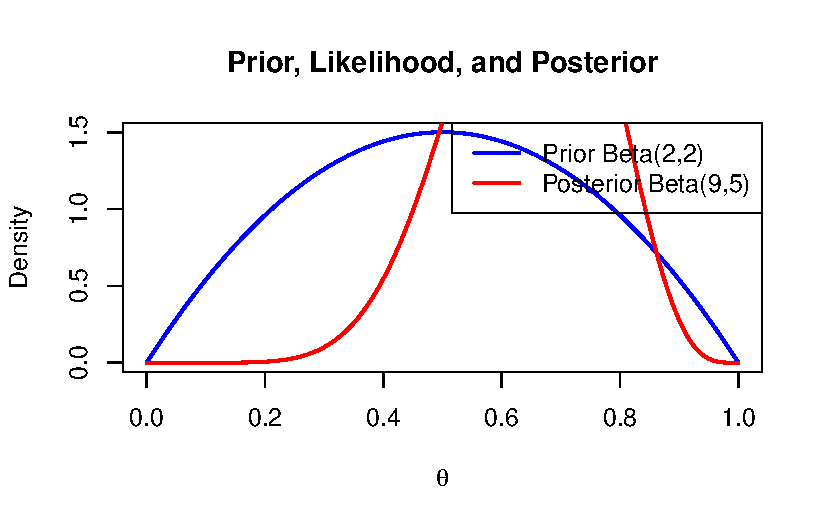
\includegraphics[keepaspectratio]{week01_files/figure-pdf/unnamed-chunk-1-1.pdf}}

\bookmarksetup{startatroot}

\chapter{Week 2 --- Conjugate Priors and Analytical
Posteriors}\label{week-2-conjugate-priors-and-analytical-posteriors}

\begin{center}\rule{0.5\linewidth}{0.5pt}\end{center}

\section{Overview}\label{overview}

This week focuses on \textbf{conjugate priors} --- special priors that
yield posteriors in the same family of distributions as the prior.\\
Students will learn why conjugacy simplifies Bayesian inference, how to
identify conjugate pairs for common likelihoods, and how to perform
analytical posterior updates without simulation.\\
We will also introduce the concept of prior sensitivity analysis and
noninformative (objective) priors.

\begin{center}\rule{0.5\linewidth}{0.5pt}\end{center}

\section{Learning Goals}\label{learning-goals}

By the end of Week 2, you should be able to:

\begin{itemize}
\tightlist
\item
  Define and identify conjugate priors for standard likelihood models.\\
\item
  Derive analytical posteriors for Binomial, Poisson, and Normal
  models.\\
\item
  Compute posterior summaries and predictive distributions.\\
\item
  Discuss the influence of priors on posterior inference.\\
\item
  Perform prior sensitivity analysis in R.
\end{itemize}

\begin{center}\rule{0.5\linewidth}{0.5pt}\end{center}

\section{Lecture 1: The Concept of
Conjugacy}\label{lecture-1-the-concept-of-conjugacy}

\subsection{1.1 Definition}\label{definition}

A \textbf{conjugate prior} for a likelihood \(p(y \mid \theta)\) is a
prior distribution \(p(\theta)\) such that the posterior
\(p(\theta \mid y)\) belongs to the same family as the prior.

Formally: \[
p(\theta \mid y) \propto p(y \mid \theta)\, p(\theta)
\] If \(p(\theta \mid y)\) has the same functional form as
\(p(\theta)\), then \(p(\theta)\) is \emph{conjugate} to the likelihood.

\subsection{1.2 Why Conjugacy Matters}\label{why-conjugacy-matters}

\begin{itemize}
\tightlist
\item
  Provides closed-form expressions for posterior means, variances, and
  credible intervals.\\
\item
  Facilitates sequential updating --- easy to update priors as new data
  arrive.\\
\item
  Useful for educational and analytic illustration before moving to MCMC
  methods.
\end{itemize}

\subsection{1.3 Examples of Conjugate
Pairs}\label{examples-of-conjugate-pairs}

\begin{longtable}[]{@{}
  >{\raggedright\arraybackslash}p{(\linewidth - 4\tabcolsep) * \real{0.2708}}
  >{\raggedright\arraybackslash}p{(\linewidth - 4\tabcolsep) * \real{0.3542}}
  >{\raggedright\arraybackslash}p{(\linewidth - 4\tabcolsep) * \real{0.3750}}@{}}
\toprule\noalign{}
\begin{minipage}[b]{\linewidth}\raggedright
Likelihood
\end{minipage} & \begin{minipage}[b]{\linewidth}\raggedright
Conjugate Prior
\end{minipage} & \begin{minipage}[b]{\linewidth}\raggedright
Posterior Family
\end{minipage} \\
\midrule\noalign{}
\endhead
\bottomrule\noalign{}
\endlastfoot
Binomial\((n,\theta)\) & Beta\((\alpha,\beta)\) &
Beta\((\alpha+y, \beta+n-y)\) \\
Poisson\((\lambda)\) & Gamma\((a,b)\) & Gamma\((a+\sum y_i, b+n)\) \\
Normal\((\mu,\sigma^2)\) (known variance) & Normal\((\mu_0,\tau_0^2)\) &
Normal\((\mu_1,\tau_1^2)\) \\
Exponential\((\lambda)\) & Gamma\((a,b)\) &
Gamma\((a+n, b+\sum y_i)\) \\
Normal mean/variance (unknown \(\sigma^2\)) & Normal--Inverse-Gamma &
Normal--Inverse-Gamma \\
\end{longtable}

\begin{center}\rule{0.5\linewidth}{0.5pt}\end{center}

\section{Lecture 2: Beta--Binomial and Gamma--Poisson
Models}\label{lecture-2-betabinomial-and-gammapoisson-models}

\subsection{2.1 Beta--Binomial Model (Review and
Generalization)}\label{betabinomial-model-review-and-generalization}

Let \(y \mid \theta \sim \text{Binomial}(n,\theta)\) and
\(\theta \sim \text{Beta}(\alpha_0,\beta_0)\).\\
Then the posterior is: \[
\theta \mid y \sim \text{Beta}(\alpha_0 + y, \beta_0 + n - y).
\]

\textbf{Posterior Mean:} \[
E[\theta \mid y] = \frac{\alpha_0 + y}{\alpha_0 + \beta_0 + n}.
\]

\textbf{Predictive Probability for a Future Success:} \[
p(\tilde{y}=1 \mid y) = E[\theta \mid y].
\]

\textbf{Interpretation:}\\
Each observation updates the Beta prior by adding one success or failure
to the corresponding shape parameter.

\begin{center}\rule{0.5\linewidth}{0.5pt}\end{center}

\subsection{2.2 Gamma--Poisson Model
(Counts)}\label{gammapoisson-model-counts}

Suppose we model count data as \(y_i \sim \text{Poisson}(\lambda)\),
with prior \(\lambda \sim \text{Gamma}(a_0, b_0)\)\\
(where the Gamma density is parameterized as
\(p(\lambda) \propto \lambda^{a_0-1} e^{-b_0\lambda}\)).

\textbf{Posterior:} \[
\lambda \mid y_1,\ldots,y_n \sim \text{Gamma}\left(a_0 + \sum_{i=1}^n y_i,\; b_0 + n\right).
\]

\textbf{Posterior Mean and Variance:} \[
E[\lambda \mid y] = \frac{a_0 + \sum y_i}{b_0 + n}, \quad
\text{Var}[\lambda \mid y] = \frac{a_0 + \sum y_i}{(b_0 + n)^2}.
\]

\textbf{Posterior Predictive:} \[
p(\tilde{y} \mid y) = \int \text{Poisson}(\tilde{y} \mid \lambda)\, p(\lambda \mid y)\, d\lambda,
\] which follows a \textbf{Negative Binomial} distribution.

\textbf{Interpretation:}\\
The Gamma prior acts as if we had observed \(a_0-1\) pseudo-events over
\(b_0\) pseudo-trials.

\begin{center}\rule{0.5\linewidth}{0.5pt}\end{center}

\subsection{2.3 R Example: Gamma--Poisson
Updating}\label{r-example-gammapoisson-updating}

\begin{Shaded}
\begin{Highlighting}[]
\CommentTok{\# Posterior update for Gamma{-}Poisson model}
\NormalTok{y }\OtherTok{\textless{}{-}} \FunctionTok{c}\NormalTok{(}\DecValTok{3}\NormalTok{, }\DecValTok{2}\NormalTok{, }\DecValTok{4}\NormalTok{, }\DecValTok{1}\NormalTok{, }\DecValTok{0}\NormalTok{, }\DecValTok{2}\NormalTok{, }\DecValTok{3}\NormalTok{)}
\NormalTok{a0 }\OtherTok{\textless{}{-}} \DecValTok{2}\NormalTok{; b0 }\OtherTok{\textless{}{-}} \DecValTok{1}   \CommentTok{\# prior Gamma(2,1)}
\NormalTok{n }\OtherTok{\textless{}{-}} \FunctionTok{length}\NormalTok{(y)}

\NormalTok{a1 }\OtherTok{\textless{}{-}}\NormalTok{ a0 }\SpecialCharTok{+} \FunctionTok{sum}\NormalTok{(y)}
\NormalTok{b1 }\OtherTok{\textless{}{-}}\NormalTok{ b0 }\SpecialCharTok{+}\NormalTok{ n}

\NormalTok{lambda }\OtherTok{\textless{}{-}} \FunctionTok{seq}\NormalTok{(}\DecValTok{0}\NormalTok{, }\DecValTok{10}\NormalTok{, }\AttributeTok{length.out =} \DecValTok{400}\NormalTok{)}
\NormalTok{prior }\OtherTok{\textless{}{-}} \FunctionTok{dgamma}\NormalTok{(lambda, a0, b0)}
\NormalTok{posterior }\OtherTok{\textless{}{-}} \FunctionTok{dgamma}\NormalTok{(lambda, a1, b1)}

\FunctionTok{plot}\NormalTok{(lambda, prior, }\AttributeTok{type=}\StringTok{"l"}\NormalTok{, }\AttributeTok{lwd=}\DecValTok{2}\NormalTok{, }\AttributeTok{col=}\StringTok{"blue"}\NormalTok{, }\AttributeTok{ylim=}\FunctionTok{c}\NormalTok{(}\DecValTok{0}\NormalTok{, }\FunctionTok{max}\NormalTok{(posterior)),}
     \AttributeTok{ylab=}\StringTok{"Density"}\NormalTok{, }\AttributeTok{xlab=}\FunctionTok{expression}\NormalTok{(lambda),}
     \AttributeTok{main=}\StringTok{"Gamma{-}Poisson Updating"}\NormalTok{)}
\FunctionTok{lines}\NormalTok{(lambda, posterior, }\AttributeTok{col=}\StringTok{"red"}\NormalTok{, }\AttributeTok{lwd=}\DecValTok{2}\NormalTok{)}
\FunctionTok{legend}\NormalTok{(}\StringTok{"topright"}\NormalTok{,}
       \AttributeTok{legend=}\FunctionTok{c}\NormalTok{(}\StringTok{"Prior Gamma(2,1)"}\NormalTok{, }\FunctionTok{paste0}\NormalTok{(}\StringTok{"Posterior Gamma("}\NormalTok{, a1, }\StringTok{","}\NormalTok{, b1, }\StringTok{")"}\NormalTok{)),}
       \AttributeTok{col=}\FunctionTok{c}\NormalTok{(}\StringTok{"blue"}\NormalTok{, }\StringTok{"red"}\NormalTok{), }\AttributeTok{lwd=}\DecValTok{2}\NormalTok{)}
\end{Highlighting}
\end{Shaded}

\pandocbounded{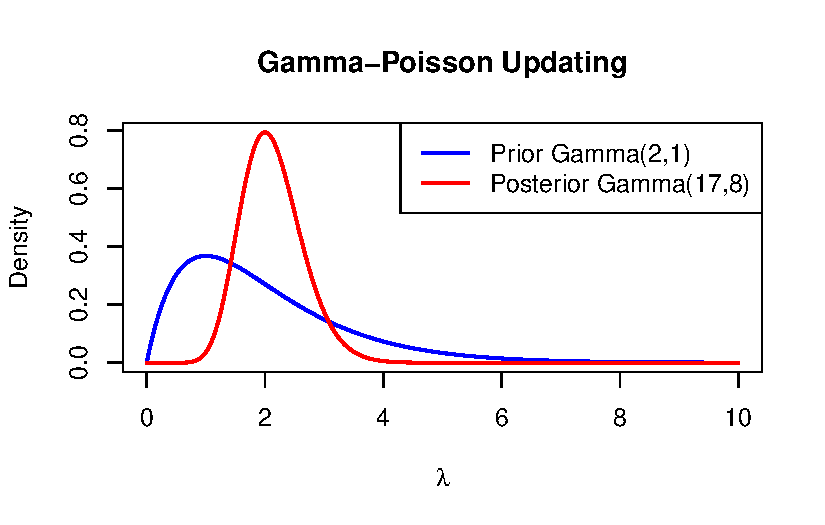
\includegraphics[keepaspectratio]{week02_files/figure-pdf/unnamed-chunk-1-1.pdf}}

\bookmarksetup{startatroot}

\chapter{Week 3 --- Monte Carlo Integration and Simulation-Based
Bayesian
Inference}\label{week-3-monte-carlo-integration-and-simulation-based-bayesian-inference}

\begin{center}\rule{0.5\linewidth}{0.5pt}\end{center}

\section{Overview}\label{overview-1}

This week introduces \textbf{Monte Carlo methods}, which allow us to
approximate Bayesian quantities when analytical solutions are
unavailable.\\
We explore how random sampling can be used to estimate expectations,
posterior summaries, and probabilities.\\
By the end of this week, students will understand how Monte Carlo
simulation forms the foundation for modern Bayesian computation such as
MCMC.

\begin{center}\rule{0.5\linewidth}{0.5pt}\end{center}

\section{Learning Goals}\label{learning-goals-1}

By the end of Week 3, you should be able to:

\begin{itemize}
\tightlist
\item
  Explain the motivation for Monte Carlo methods in Bayesian
  inference.\\
\item
  Approximate expectations, integrals, and posterior summaries using
  random sampling.\\
\item
  Implement crude Monte Carlo and importance sampling in R.\\
\item
  Assess the accuracy and variance of Monte Carlo estimators.\\
\item
  Interpret Monte Carlo errors and convergence diagnostics.
\end{itemize}

\begin{center}\rule{0.5\linewidth}{0.5pt}\end{center}

\section{Lecture 1: Motivation and Fundamentals of Monte
Carlo}\label{lecture-1-motivation-and-fundamentals-of-monte-carlo}

\subsection{1.1 The Problem}\label{the-problem}

Bayesian inference often requires evaluating integrals such as: \[
E[h(\theta) \mid y] = \int h(\theta)\, p(\theta \mid y)\, d\theta,
\] which are rarely available in closed form.

\subsection{1.2 Monte Carlo Idea}\label{monte-carlo-idea}

If we can sample \(\theta^{(1)}, \ldots, \theta^{(M)}\) from the
posterior \(p(\theta \mid y)\),\\
then we can approximate the expectation by: \[
\hat{E}[h(\theta)] = \frac{1}{M} \sum_{m=1}^M h(\theta^{(m)}).
\] This is called the \textbf{Monte Carlo estimator}.

By the \textbf{Law of Large Numbers},
\(\hat{E}[h(\theta)] \to E[h(\theta)]\) as \(M \to \infty\).\\
The \textbf{Central Limit Theorem} gives: \[
\sqrt{M}\,(\hat{E} - E[h(\theta)]) \approx N(0, \text{Var}[h(\theta)]).
\]

\subsection{1.3 Monte Carlo Error}\label{monte-carlo-error}

We can estimate the simulation error by: \[
\text{SE}(\hat{E}) \approx \sqrt{\frac{\text{Var}(h(\theta))}{M}}.
\] Larger \(M\) gives more accurate approximations but increases
computation time.

\subsection{1.4 Simple Example}\label{simple-example}

Compute \(E[\theta]\) for \(\theta \sim \text{Beta}(2,5)\) using Monte
Carlo.

\begin{Shaded}
\begin{Highlighting}[]
\FunctionTok{set.seed}\NormalTok{(}\DecValTok{1}\NormalTok{)}
\NormalTok{M }\OtherTok{\textless{}{-}} \FloatTok{1e5}
\NormalTok{theta }\OtherTok{\textless{}{-}} \FunctionTok{rbeta}\NormalTok{(M, }\DecValTok{2}\NormalTok{, }\DecValTok{5}\NormalTok{)}
\FunctionTok{mean}\NormalTok{(theta)          }\CommentTok{\# Monte Carlo estimate}
\end{Highlighting}
\end{Shaded}

\begin{verbatim}
[1] 0.2861808
\end{verbatim}

\begin{Shaded}
\begin{Highlighting}[]
\FunctionTok{var}\NormalTok{(theta) }\SpecialCharTok{/}\NormalTok{ M       }\CommentTok{\# Monte Carlo variance}
\end{Highlighting}
\end{Shaded}

\begin{verbatim}
[1] 2.56548e-07
\end{verbatim}

\bookmarksetup{startatroot}

\chapter{Week 4 --- Markov Chain Monte Carlo (MCMC)
Methods}\label{week-4-markov-chain-monte-carlo-mcmc-methods}

\begin{center}\rule{0.5\linewidth}{0.5pt}\end{center}

\section{Overview}\label{overview-2}

This week introduces \textbf{Markov Chain Monte Carlo (MCMC)} --- a
powerful class of algorithms for simulating from complex posterior
distributions that are difficult to sample from directly.\\
You will learn the logic of constructing Markov chains with a desired
stationary distribution, how to implement the Metropolis--Hastings (MH)
and Gibbs samplers, and how to assess convergence and mixing of MCMC
chains.

\begin{center}\rule{0.5\linewidth}{0.5pt}\end{center}

\section{Learning Goals}\label{learning-goals-2}

By the end of Week 4, you should be able to:

\begin{itemize}
\tightlist
\item
  Explain the intuition behind MCMC and why it works.\\
\item
  Implement simple Metropolis--Hastings and Gibbs algorithms in R.\\
\item
  Diagnose convergence using trace plots and summary statistics.\\
\item
  Compute posterior means, variances, and credible intervals from MCMC
  samples.\\
\item
  Understand practical issues such as burn-in, thinning, and
  autocorrelation.
\end{itemize}

\begin{center}\rule{0.5\linewidth}{0.5pt}\end{center}

\section{Lecture 1: Introduction to
MCMC}\label{lecture-1-introduction-to-mcmc}

\subsection{1.1 Motivation}\label{motivation}

For many posteriors, sampling directly is infeasible.\\
We instead build a \emph{Markov chain} whose stationary distribution is
the target posterior \(p(\theta \mid y)\).\\
After sufficient iterations, the draws from the chain behave like
samples from the true posterior.

\subsection{1.2 Markov Chain Basics}\label{markov-chain-basics}

A Markov chain \(\{\theta^{(t)}\}\) has the \textbf{Markov property}: \[
p(\theta^{(t)} \mid \theta^{(t-1)}, \ldots, \theta^{(1)}) = p(\theta^{(t)} \mid \theta^{(t-1)}).
\] If the chain is \textbf{ergodic}, the distribution of
\(\theta^{(t)}\) converges to a stationary distribution \(\pi(\theta)\).

MCMC constructs such chains so that \(\pi(\theta) = p(\theta \mid y)\).

\subsection{1.3 Core Idea}\label{core-idea}

Repeatedly propose a new value \(\theta^\*\) and decide whether to
\textbf{accept} or \textbf{reject} it\\
based on how likely it is under the posterior.\\
This ensures that samples eventually represent the posterior
distribution.

\begin{center}\rule{0.5\linewidth}{0.5pt}\end{center}

\section{Lecture 2: The Metropolis--Hastings
Algorithm}\label{lecture-2-the-metropolishastings-algorithm}

\subsection{2.1 Algorithm Steps}\label{algorithm-steps}

\begin{enumerate}
\def\labelenumi{\arabic{enumi}.}
\tightlist
\item
  Initialize with \(\theta^{(0)}\).\\
\item
  For each iteration \(t=1,2,\ldots,T\):

  \begin{enumerate}
  \def\labelenumii{\alph{enumii}.}
  \tightlist
  \item
    Propose \(\theta^\* \sim q(\theta^\* \mid \theta^{(t-1)})\).\\
  \item
    Compute the \textbf{acceptance probability}: \[
    \alpha = \min\left(1,\;
    \frac{p(y \mid \theta^\*)\, p(\theta^\*)\, q(\theta^{(t-1)} \mid \theta^\*)}
         {p(y \mid \theta^{(t-1)})\, p(\theta^{(t-1)})\, q(\theta^\* \mid \theta^{(t-1)})}
    \right).
    \]
  \item
    Accept \(\theta^\*\) with probability \(\alpha\); otherwise, keep
    \(\theta^{(t)} = \theta^{(t-1)}\).
  \end{enumerate}
\item
  After burn-in, the samples \(\{\theta^{(t)}\}\) approximate draws from
  \(p(\theta \mid y)\).
\end{enumerate}

\subsection{2.2 Special Case: Symmetric
Proposal}\label{special-case-symmetric-proposal}

If
\(q(\theta^\* \mid \theta^{(t-1)}) = q(\theta^{(t-1)} \mid \theta^\*)\),\\
then \[
\alpha = \min\left(1,\; \frac{p(y \mid \theta^\*)\, p(\theta^\*)}
                         {p(y \mid \theta^{(t-1)})\, p(\theta^{(t-1)})}\right).
\] This is the \textbf{Metropolis algorithm}.

\subsection{2.3 Example: Posterior for a Normal Mean (Unknown Mean,
Known
Variance)}\label{example-posterior-for-a-normal-mean-unknown-mean-known-variance}

Let \(y_i \sim N(\mu, 1)\) for \(i=1,\ldots,n\) and prior
\(\mu \sim N(0,10^2)\).

\begin{Shaded}
\begin{Highlighting}[]
\FunctionTok{set.seed}\NormalTok{(}\DecValTok{123}\NormalTok{)}
\CommentTok{\# Data}
\NormalTok{y }\OtherTok{\textless{}{-}} \FunctionTok{rnorm}\NormalTok{(}\DecValTok{50}\NormalTok{, }\AttributeTok{mean =} \DecValTok{3}\NormalTok{, }\AttributeTok{sd =} \DecValTok{1}\NormalTok{)}
\NormalTok{n }\OtherTok{\textless{}{-}} \FunctionTok{length}\NormalTok{(y)}
\NormalTok{post\_log }\OtherTok{\textless{}{-}} \ControlFlowTok{function}\NormalTok{(mu) \{}
  \FunctionTok{sum}\NormalTok{(}\FunctionTok{dnorm}\NormalTok{(y, mu, }\DecValTok{1}\NormalTok{, }\AttributeTok{log=}\ConstantTok{TRUE}\NormalTok{)) }\SpecialCharTok{+} \FunctionTok{dnorm}\NormalTok{(mu, }\DecValTok{0}\NormalTok{, }\DecValTok{10}\NormalTok{, }\AttributeTok{log=}\ConstantTok{TRUE}\NormalTok{)}
\NormalTok{\}}

\CommentTok{\# Metropolis sampler}
\NormalTok{T }\OtherTok{\textless{}{-}} \DecValTok{10000}
\NormalTok{mu }\OtherTok{\textless{}{-}} \FunctionTok{numeric}\NormalTok{(T)}
\NormalTok{mu[}\DecValTok{1}\NormalTok{] }\OtherTok{\textless{}{-}} \DecValTok{0}
\NormalTok{proposal\_sd }\OtherTok{\textless{}{-}} \FloatTok{0.5}

\ControlFlowTok{for}\NormalTok{(t }\ControlFlowTok{in} \DecValTok{2}\SpecialCharTok{:}\NormalTok{T) \{}
\NormalTok{  mu\_star }\OtherTok{\textless{}{-}} \FunctionTok{rnorm}\NormalTok{(}\DecValTok{1}\NormalTok{, mu[t}\DecValTok{{-}1}\NormalTok{], proposal\_sd)}
\NormalTok{  log\_alpha }\OtherTok{\textless{}{-}} \FunctionTok{post\_log}\NormalTok{(mu\_star) }\SpecialCharTok{{-}} \FunctionTok{post\_log}\NormalTok{(mu[t}\DecValTok{{-}1}\NormalTok{])}
  \ControlFlowTok{if}\NormalTok{(}\FunctionTok{log}\NormalTok{(}\FunctionTok{runif}\NormalTok{(}\DecValTok{1}\NormalTok{)) }\SpecialCharTok{\textless{}}\NormalTok{ log\_alpha) mu[t] }\OtherTok{\textless{}{-}}\NormalTok{ mu\_star }\ControlFlowTok{else}\NormalTok{ mu[t] }\OtherTok{\textless{}{-}}\NormalTok{ mu[t}\DecValTok{{-}1}\NormalTok{]}
\NormalTok{\}}

\NormalTok{burnin }\OtherTok{\textless{}{-}} \DecValTok{1000}
\NormalTok{post\_samples }\OtherTok{\textless{}{-}}\NormalTok{ mu[(burnin}\SpecialCharTok{+}\DecValTok{1}\NormalTok{)}\SpecialCharTok{:}\NormalTok{T]}

\FunctionTok{hist}\NormalTok{(post\_samples, }\AttributeTok{prob=}\ConstantTok{TRUE}\NormalTok{, }\AttributeTok{col=}\StringTok{"skyblue"}\NormalTok{, }\AttributeTok{main=}\StringTok{"Posterior Samples for μ"}\NormalTok{)}
\FunctionTok{abline}\NormalTok{(}\AttributeTok{v =} \FunctionTok{mean}\NormalTok{(post\_samples), }\AttributeTok{col=}\StringTok{"red"}\NormalTok{, }\AttributeTok{lwd=}\DecValTok{2}\NormalTok{)}
\end{Highlighting}
\end{Shaded}

\pandocbounded{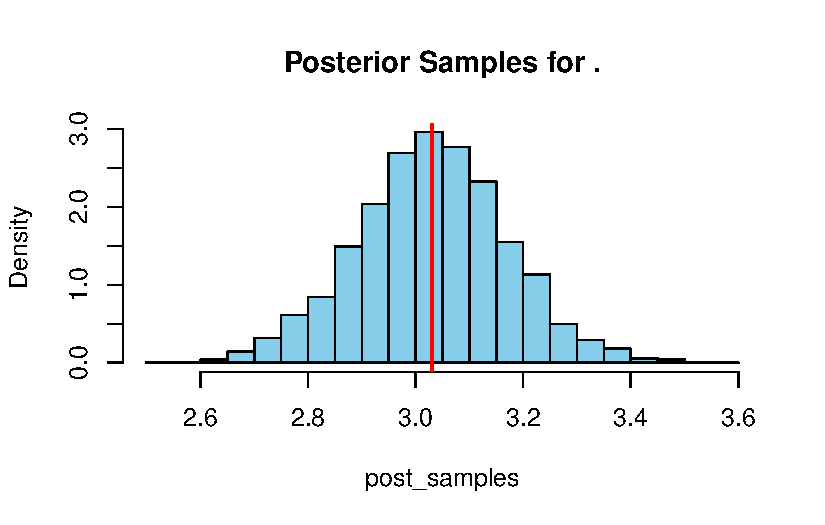
\includegraphics[keepaspectratio]{week04_files/figure-pdf/unnamed-chunk-1-1.pdf}}

\bookmarksetup{startatroot}

\chapter{Week 5 --- Model Checking and
Comparison}\label{week-5-model-checking-and-comparison}

This week introduces methods for evaluating Bayesian model adequacy and
comparing models.\\
We focus on \textbf{Posterior Predictive Checking (PPC)} and
\textbf{Bayesian Model Comparison} via Bayes factors, WAIC, and LOO.\\
Students will diagnose model fit using replicated data and compare
predictive accuracy among competing models.

\begin{center}\rule{0.5\linewidth}{0.5pt}\end{center}

\section{Learning Goals}\label{learning-goals-3}

By the end of this week, you should be able to:

\begin{itemize}
\tightlist
\item
  Generate and interpret posterior predictive distributions.\\
\item
  Use posterior predictive checks to detect model misspecification.\\
\item
  Compute and interpret WAIC, LOO, and Bayes factors.\\
\item
  Evaluate model adequacy visually and numerically in R.
\end{itemize}

\begin{center}\rule{0.5\linewidth}{0.5pt}\end{center}

\section{Lecture 1 --- Posterior Predictive
Checking}\label{lecture-1-posterior-predictive-checking}

\subsection{Posterior Predictive
Distribution}\label{posterior-predictive-distribution-1}

For data \(y\) and parameters \(\theta\), \[
p(\tilde{y}\mid y) = \int p(\tilde{y}\mid\theta)\,p(\theta\mid y)\,d\theta.
\] If a model is adequate, the observed data \(y\) should look typical
among replicated datasets \(\tilde{y}\) simulated from this
distribution.

\subsection{Implementation Steps}\label{implementation-steps}

\begin{enumerate}
\def\labelenumi{\arabic{enumi}.}
\tightlist
\item
  Choose a \textbf{discrepancy statistic} \(T(y,\theta)\) capturing an
  aspect of fit.\\
\item
  For each posterior draw \(\theta^{(m)}\):

  \begin{itemize}
  \tightlist
  \item
    Simulate \(\tilde{y}^{(m)}\!\sim\!p(\tilde{y}\mid\theta^{(m)})\).\\
  \item
    Compute \(T(y,\theta^{(m)})\) and
    \(T(\tilde{y}^{(m)},\theta^{(m)})\).\\
  \end{itemize}
\item
  Compute posterior predictive \(p\)-value:\\
  \[
  p_{\text{ppc}}=P\!\left(T(\tilde{y},\theta)\!>\!T(y,\theta)\mid y\right).
  \]
\end{enumerate}

Values near 0 or 1 suggest lack of fit.

\subsection{Example A --- Binomial
Model}\label{example-a-binomial-model}

\begin{Shaded}
\begin{Highlighting}[]
\FunctionTok{set.seed}\NormalTok{(}\DecValTok{5}\NormalTok{)}
\NormalTok{M }\OtherTok{\textless{}{-}} \DecValTok{5000}
\NormalTok{y\_obs }\OtherTok{\textless{}{-}} \DecValTok{7}\NormalTok{; n }\OtherTok{\textless{}{-}} \DecValTok{10}

\NormalTok{theta }\OtherTok{\textless{}{-}} \FunctionTok{rbeta}\NormalTok{(M, }\DecValTok{2} \SpecialCharTok{+}\NormalTok{ y\_obs, }\DecValTok{2} \SpecialCharTok{+}\NormalTok{ n }\SpecialCharTok{{-}}\NormalTok{ y\_obs)   }\CommentTok{\# posterior draws}
\NormalTok{y\_rep }\OtherTok{\textless{}{-}} \FunctionTok{rbinom}\NormalTok{(M, n, theta)}

\NormalTok{ppc\_p }\OtherTok{\textless{}{-}} \FunctionTok{mean}\NormalTok{(y\_rep }\SpecialCharTok{\textgreater{}=}\NormalTok{ y\_obs)}
\NormalTok{ppc\_p}
\end{Highlighting}
\end{Shaded}

\begin{verbatim}
[1] 0.509
\end{verbatim}

\begin{Shaded}
\begin{Highlighting}[]
\FunctionTok{hist}\NormalTok{(y\_rep, }\AttributeTok{breaks=}\FunctionTok{seq}\NormalTok{(}\SpecialCharTok{{-}}\FloatTok{0.5}\NormalTok{, n}\FloatTok{+0.5}\NormalTok{, }\AttributeTok{by=}\DecValTok{1}\NormalTok{),}
     \AttributeTok{col=}\StringTok{"skyblue"}\NormalTok{, }\AttributeTok{main=}\StringTok{"Posterior Predictive Distribution"}\NormalTok{, }\AttributeTok{xlab=}\StringTok{"Replicated ỹ"}\NormalTok{)}
\FunctionTok{abline}\NormalTok{(}\AttributeTok{v=}\NormalTok{y\_obs, }\AttributeTok{col=}\StringTok{"red"}\NormalTok{, }\AttributeTok{lwd=}\DecValTok{2}\NormalTok{)}
\FunctionTok{legend}\NormalTok{(}\StringTok{"topright"}\NormalTok{, }\AttributeTok{legend=}\FunctionTok{c}\NormalTok{(}\StringTok{"Observed y"}\NormalTok{), }\AttributeTok{col=}\StringTok{"red"}\NormalTok{, }\AttributeTok{lwd=}\DecValTok{2}\NormalTok{, }\AttributeTok{bty=}\StringTok{"n"}\NormalTok{)}
\end{Highlighting}
\end{Shaded}

\begin{figure}[H]

{\centering \pandocbounded{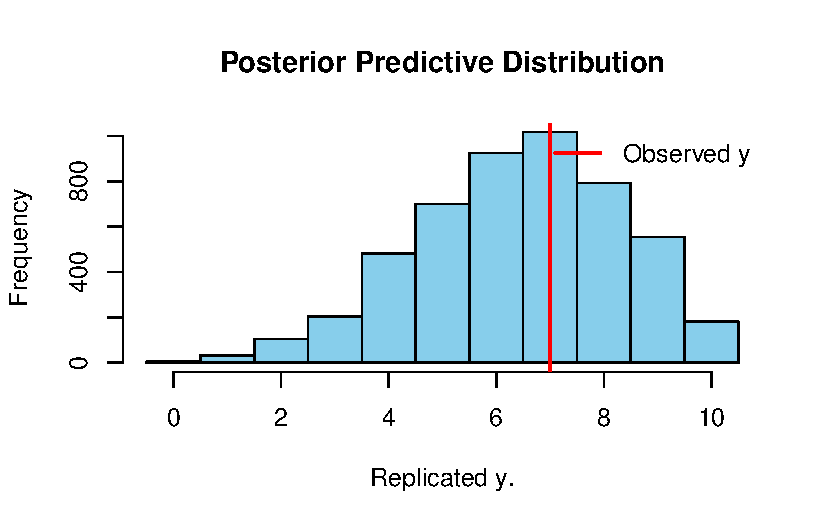
\includegraphics[keepaspectratio]{week05_files/figure-pdf/ppc-binomial-plot-1.pdf}}

}

\caption{Posterior predictive distribution of ỹ}

\end{figure}%

\subsection{Example B --- Normal Model (Standard Deviation
Check)}\label{example-b-normal-model-standard-deviation-check}

\begin{Shaded}
\begin{Highlighting}[]
\FunctionTok{set.seed}\NormalTok{(}\DecValTok{6}\NormalTok{)}
\NormalTok{y }\OtherTok{\textless{}{-}} \FunctionTok{rnorm}\NormalTok{(}\DecValTok{30}\NormalTok{, }\AttributeTok{mean=}\DecValTok{0}\NormalTok{, }\AttributeTok{sd=}\DecValTok{1}\NormalTok{)}
\NormalTok{mu\_draw }\OtherTok{\textless{}{-}} \FunctionTok{rnorm}\NormalTok{(}\DecValTok{1000}\NormalTok{, }\DecValTok{0}\NormalTok{, }\DecValTok{1}\NormalTok{)}
\NormalTok{y\_rep\_mat }\OtherTok{\textless{}{-}} \FunctionTok{replicate}\NormalTok{(}\DecValTok{200}\NormalTok{, }\FunctionTok{rnorm}\NormalTok{(}\FunctionTok{length}\NormalTok{(y), }\FunctionTok{sample}\NormalTok{(mu\_draw,}\DecValTok{1}\NormalTok{), }\DecValTok{1}\NormalTok{))}

\NormalTok{T\_obs }\OtherTok{\textless{}{-}} \FunctionTok{sd}\NormalTok{(y)}
\NormalTok{T\_rep }\OtherTok{\textless{}{-}} \FunctionTok{apply}\NormalTok{(y\_rep\_mat, }\DecValTok{2}\NormalTok{, sd)}

\FunctionTok{mean}\NormalTok{(T\_rep }\SpecialCharTok{\textgreater{}=}\NormalTok{ T\_obs)}
\end{Highlighting}
\end{Shaded}

\begin{verbatim}
[1] 0.145
\end{verbatim}

\begin{Shaded}
\begin{Highlighting}[]
\FunctionTok{hist}\NormalTok{(T\_rep, }\AttributeTok{col=}\StringTok{"lightgray"}\NormalTok{, }\AttributeTok{main=}\StringTok{"Posterior Predictive Check: SD"}\NormalTok{,}
     \AttributeTok{xlab=}\StringTok{"Replicated sd(ỹ)"}\NormalTok{)}
\FunctionTok{abline}\NormalTok{(}\AttributeTok{v=}\NormalTok{T\_obs, }\AttributeTok{col=}\StringTok{"red"}\NormalTok{, }\AttributeTok{lwd=}\DecValTok{2}\NormalTok{)}
\FunctionTok{legend}\NormalTok{(}\StringTok{"topright"}\NormalTok{, }\AttributeTok{legend=}\FunctionTok{c}\NormalTok{(}\StringTok{"Observed sd(y)"}\NormalTok{), }\AttributeTok{col=}\StringTok{"red"}\NormalTok{, }\AttributeTok{lwd=}\DecValTok{2}\NormalTok{, }\AttributeTok{bty=}\StringTok{"n"}\NormalTok{)}
\end{Highlighting}
\end{Shaded}

\begin{figure}[H]

{\centering \pandocbounded{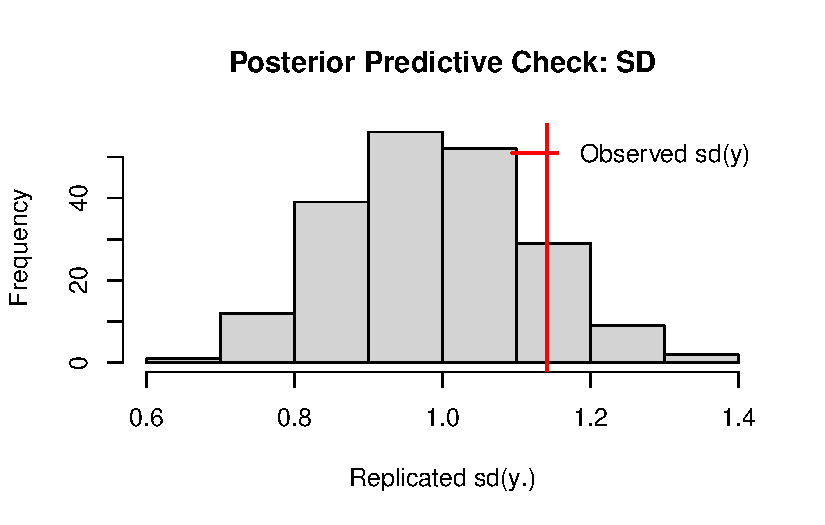
\includegraphics[keepaspectratio]{week05_files/figure-pdf/ppc-normal-plot-1.pdf}}

}

\caption{PPC for sample standard deviation}

\end{figure}%

\subsection{Practical Tips}\label{practical-tips}

\begin{itemize}
\tightlist
\item
  Use \textbf{multiple} statistics (\(T_1, T_2,\dots\)).\\
\item
  Visual checks often outperform a single numeric \(p_{\text{ppc}}\).\\
\item
  Integrate PPC with subject-matter knowledge and residual plots.
\end{itemize}

\begin{center}\rule{0.5\linewidth}{0.5pt}\end{center}

\section{Lecture 2 --- Bayesian Model
Comparison}\label{lecture-2-bayesian-model-comparison}

\subsection{Motivation}\label{motivation-1}

Competing Bayesian models are compared by their fit and complexity.\\
Common approaches include \textbf{Bayes factors}, \textbf{WAIC}, and
\textbf{LOO}.

\begin{center}\rule{0.5\linewidth}{0.5pt}\end{center}

\subsection{Bayes Factors}\label{bayes-factors}

Given two models \(M_1\) and \(M_2\), \[
\text{BF}_{12} = \frac{p(y\mid M_1)}{p(y\mid M_2)} ,\qquad
p(y\mid M)=\int p(y\mid\theta_M,M)\,p(\theta_M\mid M)\,d\theta_M.
\] - \(\text{BF}_{12}>1\) favors \(M_1\).\\
- Express in \(\log_{10}\) scale for interpretation.

\begin{longtable}[]{@{}cl@{}}
\toprule\noalign{}
\(\log_{10}\text{BF}_{12}\) & Evidence for \(M_1\) \\
\midrule\noalign{}
\endhead
\bottomrule\noalign{}
\endlastfoot
0--0.5 & Barely worth mentioning \\
0.5--1 & Substantial \\
1--2 & Strong \\
\textgreater2 & Decisive \\
\end{longtable}

\begin{center}\rule{0.5\linewidth}{0.5pt}\end{center}

\subsection{WAIC and LOO (Predictive
Criteria)}\label{waic-and-loo-predictive-criteria}

When computing marginal likelihoods is infeasible, we use predictive
criteria:

\begin{itemize}
\item
  \textbf{WAIC (Watanabe--Akaike Information Criterion)}\\
  \[
  \text{WAIC} = -2(\text{lppd} - p_{\text{WAIC}}),
  \] where
  \(\text{lppd}=\sum_i \log\!\left(\frac{1}{S}\sum_{s=1}^S p(y_i\mid\theta^{(s)})\right)\).
\item
  \textbf{LOO (Leave-One-Out Cross-Validation)}\\
  Approximates the out-of-sample predictive performance: \[
  \text{LOO} = \sum_i \log p(y_i \mid y_{-i}),
  \] usually estimated via Pareto-smoothed importance sampling
  (PSIS-LOO).
\end{itemize}

Lower WAIC (or higher elpd\_loo) indicates better predictive
performance.

\begin{center}\rule{0.5\linewidth}{0.5pt}\end{center}

\subsection{\texorpdfstring{Example A --- Comparing Two Regression
Models with \texttt{brms} (optional heavy
computation)}{Example A --- Comparing Two Regression Models with brms (optional heavy computation)}}\label{example-a-comparing-two-regression-models-with-brms-optional-heavy-computation}

\begin{Shaded}
\begin{Highlighting}[]
\CommentTok{\# Uncomment and install if needed}
\CommentTok{\# install.packages(c("brms", "loo"))}

\FunctionTok{library}\NormalTok{(brms)}
\FunctionTok{library}\NormalTok{(loo)}

\FunctionTok{set.seed}\NormalTok{(}\DecValTok{7}\NormalTok{)}
\NormalTok{dat }\OtherTok{\textless{}{-}} \FunctionTok{data.frame}\NormalTok{(}\AttributeTok{x =} \FunctionTok{rnorm}\NormalTok{(}\DecValTok{200}\NormalTok{))}
\NormalTok{dat}\SpecialCharTok{$}\NormalTok{y }\OtherTok{\textless{}{-}} \DecValTok{2} \SpecialCharTok{+} \DecValTok{3}\SpecialCharTok{*}\NormalTok{dat}\SpecialCharTok{$}\NormalTok{x }\SpecialCharTok{+} \FloatTok{1.5}\SpecialCharTok{*}\NormalTok{dat}\SpecialCharTok{$}\NormalTok{x}\SpecialCharTok{\^{}}\DecValTok{2} \SpecialCharTok{+} \FunctionTok{rnorm}\NormalTok{(}\DecValTok{200}\NormalTok{, }\AttributeTok{sd =} \DecValTok{1}\NormalTok{)  }\CommentTok{\# true quadratic}

\CommentTok{\# Fit linear vs quadratic models}
\NormalTok{m1 }\OtherTok{\textless{}{-}} \FunctionTok{brm}\NormalTok{(y }\SpecialCharTok{\textasciitilde{}}\NormalTok{ x, }\AttributeTok{data =}\NormalTok{ dat, }\AttributeTok{family =} \FunctionTok{gaussian}\NormalTok{(), }\AttributeTok{refresh =} \DecValTok{0}\NormalTok{)}
\NormalTok{m2 }\OtherTok{\textless{}{-}} \FunctionTok{brm}\NormalTok{(y }\SpecialCharTok{\textasciitilde{}}\NormalTok{ x }\SpecialCharTok{+} \FunctionTok{I}\NormalTok{(x}\SpecialCharTok{\^{}}\DecValTok{2}\NormalTok{), }\AttributeTok{data =}\NormalTok{ dat, }\AttributeTok{family =} \FunctionTok{gaussian}\NormalTok{(), }\AttributeTok{refresh =} \DecValTok{0}\NormalTok{)}

\NormalTok{loo1 }\OtherTok{\textless{}{-}} \FunctionTok{loo}\NormalTok{(m1)}
\NormalTok{loo2 }\OtherTok{\textless{}{-}} \FunctionTok{loo}\NormalTok{(m2)}
\FunctionTok{loo\_compare}\NormalTok{(loo1, loo2)}

\FunctionTok{pp\_check}\NormalTok{(m1)}
\FunctionTok{pp\_check}\NormalTok{(m2)}
\end{Highlighting}
\end{Shaded}

\begin{center}\rule{0.5\linewidth}{0.5pt}\end{center}

\subsection{Example B --- Quick WAIC Comparison via Frequentist
Approximation}\label{example-b-quick-waic-comparison-via-frequentist-approximation}

\begin{Shaded}
\begin{Highlighting}[]
\FunctionTok{set.seed}\NormalTok{(}\DecValTok{42}\NormalTok{)}
\NormalTok{N }\OtherTok{\textless{}{-}} \DecValTok{150}
\NormalTok{x }\OtherTok{\textless{}{-}} \FunctionTok{rnorm}\NormalTok{(N)}
\NormalTok{y }\OtherTok{\textless{}{-}} \FloatTok{1.5} \SpecialCharTok{+} \FloatTok{2.2}\SpecialCharTok{*}\NormalTok{x }\SpecialCharTok{+} \FunctionTok{rnorm}\NormalTok{(N, }\AttributeTok{sd=}\FloatTok{1.2}\NormalTok{)}

\NormalTok{m1 }\OtherTok{\textless{}{-}} \FunctionTok{lm}\NormalTok{(y }\SpecialCharTok{\textasciitilde{}}\NormalTok{ x)}
\NormalTok{m2 }\OtherTok{\textless{}{-}} \FunctionTok{lm}\NormalTok{(y }\SpecialCharTok{\textasciitilde{}} \FunctionTok{poly}\NormalTok{(x, }\DecValTok{2}\NormalTok{, }\AttributeTok{raw =} \ConstantTok{TRUE}\NormalTok{))}

\NormalTok{sigma1 }\OtherTok{\textless{}{-}} \FunctionTok{summary}\NormalTok{(m1)}\SpecialCharTok{$}\NormalTok{sigma}
\NormalTok{sigma2 }\OtherTok{\textless{}{-}} \FunctionTok{summary}\NormalTok{(m2)}\SpecialCharTok{$}\NormalTok{sigma}

\CommentTok{\# Pseudo{-}WAIC: approximate lppd {-} 2p using residual sum of squares}
\NormalTok{RSS1 }\OtherTok{\textless{}{-}} \FunctionTok{sum}\NormalTok{(}\FunctionTok{resid}\NormalTok{(m1)}\SpecialCharTok{\^{}}\DecValTok{2}\NormalTok{)}
\NormalTok{RSS2 }\OtherTok{\textless{}{-}} \FunctionTok{sum}\NormalTok{(}\FunctionTok{resid}\NormalTok{(m2)}\SpecialCharTok{\^{}}\DecValTok{2}\NormalTok{)}
\NormalTok{npar1 }\OtherTok{\textless{}{-}} \FunctionTok{length}\NormalTok{(}\FunctionTok{coef}\NormalTok{(m1))}
\NormalTok{npar2 }\OtherTok{\textless{}{-}} \FunctionTok{length}\NormalTok{(}\FunctionTok{coef}\NormalTok{(m2))}

\NormalTok{WAIC1 }\OtherTok{\textless{}{-}} \SpecialCharTok{{-}}\DecValTok{2} \SpecialCharTok{*}\NormalTok{ (}\FunctionTok{sum}\NormalTok{(}\FunctionTok{dnorm}\NormalTok{(y, }\FunctionTok{predict}\NormalTok{(m1), sigma1, }\AttributeTok{log=}\ConstantTok{TRUE}\NormalTok{)) }\SpecialCharTok{{-}}\NormalTok{ npar1)}
\NormalTok{WAIC2 }\OtherTok{\textless{}{-}} \SpecialCharTok{{-}}\DecValTok{2} \SpecialCharTok{*}\NormalTok{ (}\FunctionTok{sum}\NormalTok{(}\FunctionTok{dnorm}\NormalTok{(y, }\FunctionTok{predict}\NormalTok{(m2), sigma2, }\AttributeTok{log=}\ConstantTok{TRUE}\NormalTok{)) }\SpecialCharTok{{-}}\NormalTok{ npar2)}

\FunctionTok{data.frame}\NormalTok{(}\AttributeTok{Model=}\FunctionTok{c}\NormalTok{(}\StringTok{"Linear"}\NormalTok{,}\StringTok{"Quadratic"}\NormalTok{), }\AttributeTok{WAIC=}\FunctionTok{c}\NormalTok{(WAIC1,WAIC2))}
\end{Highlighting}
\end{Shaded}

\begin{verbatim}
      Model     WAIC
1    Linear 473.9530
2 Quadratic 475.7823
\end{verbatim}

\begin{center}\rule{0.5\linewidth}{0.5pt}\end{center}

\subsection{Visual Predictive
Comparison}\label{visual-predictive-comparison}

\begin{Shaded}
\begin{Highlighting}[]
\FunctionTok{plot}\NormalTok{(x, y, }\AttributeTok{pch=}\DecValTok{19}\NormalTok{, }\AttributeTok{col=}\StringTok{"\#00000055"}\NormalTok{, }\AttributeTok{main=}\StringTok{"Observed Data with Fitted Models"}\NormalTok{)}
\NormalTok{xs }\OtherTok{\textless{}{-}} \FunctionTok{seq}\NormalTok{(}\FunctionTok{min}\NormalTok{(x), }\FunctionTok{max}\NormalTok{(x), }\AttributeTok{length.out=}\DecValTok{200}\NormalTok{)}
\FunctionTok{lines}\NormalTok{(xs, }\FunctionTok{predict}\NormalTok{(m1, }\AttributeTok{newdata=}\FunctionTok{data.frame}\NormalTok{(}\AttributeTok{x=}\NormalTok{xs)), }\AttributeTok{col=}\StringTok{"steelblue"}\NormalTok{, }\AttributeTok{lwd=}\DecValTok{2}\NormalTok{)}
\FunctionTok{lines}\NormalTok{(xs, }\FunctionTok{predict}\NormalTok{(m2, }\AttributeTok{newdata=}\FunctionTok{data.frame}\NormalTok{(}\AttributeTok{x=}\NormalTok{xs)), }\AttributeTok{col=}\StringTok{"firebrick"}\NormalTok{, }\AttributeTok{lwd=}\DecValTok{2}\NormalTok{)}
\FunctionTok{legend}\NormalTok{(}\StringTok{"topleft"}\NormalTok{, }\AttributeTok{lwd=}\DecValTok{2}\NormalTok{, }\AttributeTok{col=}\FunctionTok{c}\NormalTok{(}\StringTok{"steelblue"}\NormalTok{,}\StringTok{"firebrick"}\NormalTok{),}
       \AttributeTok{legend=}\FunctionTok{c}\NormalTok{(}\StringTok{"Linear"}\NormalTok{,}\StringTok{"Quadratic"}\NormalTok{), }\AttributeTok{bty=}\StringTok{"n"}\NormalTok{)}
\end{Highlighting}
\end{Shaded}

\begin{figure}[H]

{\centering \pandocbounded{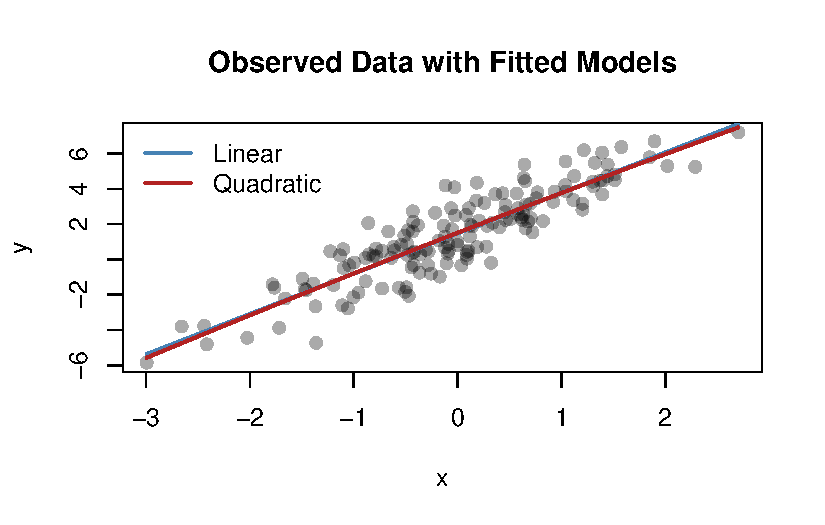
\includegraphics[keepaspectratio]{week05_files/figure-pdf/visual-overlay-1.pdf}}

}

\caption{Overlay of linear and quadratic model fits}

\end{figure}%

\begin{center}\rule{0.5\linewidth}{0.5pt}\end{center}

\subsection{Practical Summary}\label{practical-summary}

\begin{longtable}[]{@{}
  >{\raggedright\arraybackslash}p{(\linewidth - 4\tabcolsep) * \real{0.3333}}
  >{\raggedright\arraybackslash}p{(\linewidth - 4\tabcolsep) * \real{0.3333}}
  >{\raggedright\arraybackslash}p{(\linewidth - 4\tabcolsep) * \real{0.3333}}@{}}
\toprule\noalign{}
\begin{minipage}[b]{\linewidth}\raggedright
Method
\end{minipage} & \begin{minipage}[b]{\linewidth}\raggedright
Strength
\end{minipage} & \begin{minipage}[b]{\linewidth}\raggedright
Limitation
\end{minipage} \\
\midrule\noalign{}
\endhead
\bottomrule\noalign{}
\endlastfoot
Posterior Predictive Check & Diagnoses lack of fit to \textbf{observed}
data & Not inherently comparative \\
Bayes Factor & Theoretically coherent model evidence & Sensitive to
priors; hard integration \\
WAIC / LOO & Out-of-sample predictive performance & Approximate; needs
posterior draws \\
\end{longtable}

\begin{center}\rule{0.5\linewidth}{0.5pt}\end{center}

\section{Lab 5 --- Model Checking and
Comparison}\label{lab-5-model-checking-and-comparison}

\textbf{Objectives}

\begin{enumerate}
\def\labelenumi{\arabic{enumi}.}
\tightlist
\item
  Perform PPC using both numerical and visual methods.\\
\item
  Compute and interpret WAIC and LOO for model selection.\\
\item
  Visualize predictive differences among models.
\end{enumerate}

\textbf{Packages}

\texttt{brms}, \texttt{loo}, \texttt{bayesplot}, \texttt{ggplot2}

\textbf{Tasks}

\begin{itemize}
\tightlist
\item
  Fit two Bayesian regression models on the same dataset.\\
\item
  Conduct posterior predictive checks and compare simulated vs.~observed
  data.\\
\item
  Compute WAIC and LOO; summarize which model performs better.
\end{itemize}

\begin{center}\rule{0.5\linewidth}{0.5pt}\end{center}

\section{Homework 5}\label{homework-5}

\begin{enumerate}
\def\labelenumi{\arabic{enumi}.}
\tightlist
\item
  \textbf{Conceptual}

  \begin{itemize}
  \tightlist
  \item
    Explain the purpose of posterior predictive checks.\\
  \item
    Compare WAIC and LOO conceptually.
  \end{itemize}
\item
  \textbf{Computational}

  \begin{itemize}
  \tightlist
  \item
    Simulate data from a known model. Fit two Bayesian models in R.\\
  \item
    Use PPC, WAIC, and LOO to assess fit.\\
  \item
    Discuss how model choice depends on criterion used.
  \end{itemize}
\item
  \textbf{Reflection}

  \begin{itemize}
  \tightlist
  \item
    Why might visual checks and numerical metrics disagree?\\
  \item
    Which model would you report and why?
  \end{itemize}
\end{enumerate}

\begin{center}\rule{0.5\linewidth}{0.5pt}\end{center}

\section{Key Takeaways}\label{key-takeaways}

\begin{longtable}[]{@{}
  >{\raggedright\arraybackslash}p{(\linewidth - 2\tabcolsep) * \real{0.5000}}
  >{\raggedright\arraybackslash}p{(\linewidth - 2\tabcolsep) * \real{0.5000}}@{}}
\toprule\noalign{}
\begin{minipage}[b]{\linewidth}\raggedright
Concept
\end{minipage} & \begin{minipage}[b]{\linewidth}\raggedright
Summary
\end{minipage} \\
\midrule\noalign{}
\endhead
\bottomrule\noalign{}
\endlastfoot
Posterior Predictive Check & Compares observed data to replicated draws
under the posterior. \\
Posterior Predictive p-Value & Quantifies fit; extremes suggest model
misfit. \\
WAIC / LOO & Predictive performance measures for Bayesian models. \\
Bayes Factor & Ratio of marginal likelihoods for model comparison. \\
Combined Evaluation & Use graphical and numerical criteria together. \\
\end{longtable}

\begin{center}\rule{0.5\linewidth}{0.5pt}\end{center}

\textbf{Next Week:} Hierarchical Bayesian Models --- introducing partial
pooling and shrinkage.

\bookmarksetup{startatroot}

\chapter{Summary}\label{summary}

In summary, this book has no content whatsoever.

\begin{Shaded}
\begin{Highlighting}[]
\DecValTok{1} \SpecialCharTok{+} \DecValTok{1}
\end{Highlighting}
\end{Shaded}

\begin{verbatim}
[1] 2
\end{verbatim}

\bookmarksetup{startatroot}

\chapter*{References}\label{references}
\addcontentsline{toc}{chapter}{References}

\markboth{References}{References}

\phantomsection\label{refs}
\begin{CSLReferences}{1}{0}
\bibitem[\citeproctext]{ref-knuth84}
Knuth, Donald E. 1984. {``Literate Programming.''} \emph{Comput. J.} 27
(2): 97--111. \url{https://doi.org/10.1093/comjnl/27.2.97}.

\end{CSLReferences}




\end{document}
